%! suppress = MissingImport
% als een titel te lang voor 1 regel is, moet je chapterpage gebruiken (in plaats van chapter)
% Eerste geef je tussen de {} de hele titel, vervolgens tussen [] het stuk van de titel per regel
\chapterpage{Voorbeelden van het gebruik van \LaTeX}[Voorbeelden van het][gebruik van \LaTeX]
\label{ch:voorbeelden}

\section{Enkele basis \emph{environments}}
\label{sec:basis_environment}

Veel elementen in \LaTeX worden in een zogenaamde \emph{environment} gestopt.

Een voorbeeld is een opsomming met bullets:


\begin{itemize}
    \item Eerste punt dat ik wil maken
    \item Tweede punt is dit
    \item Ten slotte nog dat
\end{itemize}

Je kan een item lijst ook nesten om sub items te maken

\begin{itemize}
    \item Eerste punt dat ik wil maken
    \item Tweede punt is dit
    \begin{itemize}
        \item Voorbeeld is dat en dat
        \item Of ook wel zus en zo
    \end{itemize}
    \item Ten slotte nog dat
\end{itemize}

Als je in plaats van bullets een genummerde lijst wil maken kan \emph{enumerate} gebruiken:

\begin{enumerate}
    \item Eerste punt dat ik wil maken
    \item Tweede punt is dit
    \begin{itemize}
        \item Voorbeeld is dat en dat
        \item Of ook wel zus en zo
    \end{itemize}
    \item Ten slotte nog dat
\end{enumerate}


\section{Een plaatje toevoegen}
\label{sec:plaatje_toevoegen}

Als voorbeeld nemen we een plaatje met de afmetingen van een bloem.
De data kan je terug vinden in de Seaborn database~\citep{Waskom2021}.

We doen dit twee keer:  één keer maken we de pdf met highcharts, en één keer maken we de pdf
\emph{en} de highcharts json met Python.

\subsection{Plaatje maken met Highcharts}
\label{subsec:plaatje_highcharts}

In deze sectie laten we zien hoe je een plaatje via highcharts kan toevoegen.
Dit lijkt de eenvoudigste weg, maar vergelijken met de volgende methode, zitten hier wat meer
complicaties omdat er wat meer tussen stappen nodig zijn.
Bovendien is het eindresultaat minder mooi.

In het kort moet je de volgende stappen doen.

\begin{enumerate}
    \item Maak de csv data file waarvan je het plaatje wilt maken.
    \item Importeer de data in Highcharts en kies de juiste template
    \item Voeg alle juiste label en titels toe.
    De figuur nummer moet gelijk zijn aan het nummer zoals latex dat genereert.
    Deze moet je in highcharts handmatig toevoegen
    \item Save je project  in een json template file, zodat je later nog aanpassingen kunt maken
    \item Exporteer je plaatje als html.
    Deze ga je aan CCN leveren.
    \item Exporteer je plaatje als svg
    Deze gaan we in je latex document importeren.
    \item Open de svg file in Inkscape (open source editor) en haal de titel van je plaatje weg.
    De titel wordt namelijk door latex al geplaatst.
    \item Save je plaatje in de figures directory als svg \emph{en} als pdf
    \item De pdf file importeren we uiteindelijk in je latex document.
\end{enumerate}

% gebruik voor zowel figuren als tabellen de 'figure' environment. Op die manier delen ze de
% nummering, wat een CCN eis is. Tabel 3.1.2 volgt dan op figuur 3.1.1
\begin{figure}
    % figuren en tabellen hebben altijd een bovenschrift
    \caption{Gemiddelde afmeting per bloemonderdeel, plaatje gemaakt met highcharts}

    % direct na de caption zet je de label. Met \ref{fig:gemiddelde_afmeting} kan je vervolgens
    % naar deze figuur verwijzen in de tekst
    \label{fig:gemiddelde_afmeting_hc}

    % met \includegraphics kan je een figuur toevoegen
    % de linker kant van de figuur moet alignen met de caption. Gebruik \hspace{} om de figuur
    % zo te schuiven dat het goed is
    \hspace{-0.14cm}{
        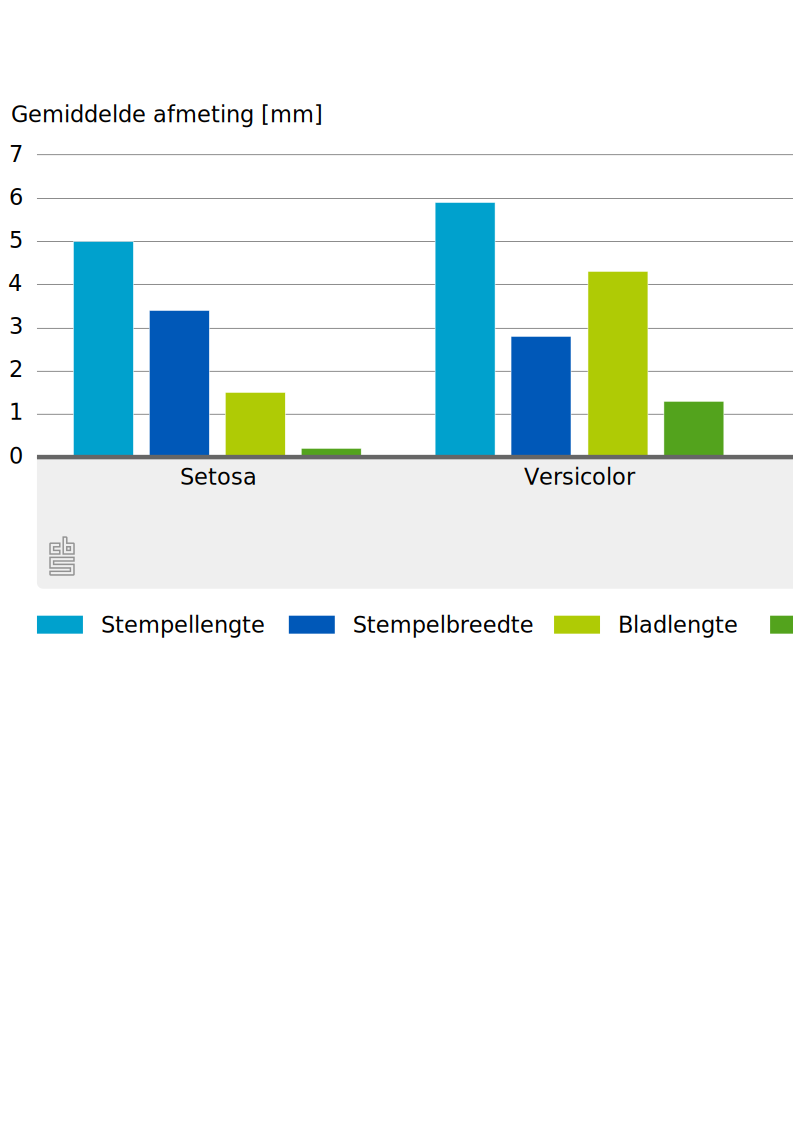
\includegraphics[width=\textwidth]{figures/iris_via_hc/afmetingen_bloem_hc}
    }
\end{figure}


Een voorbeeld van een plaatje met highcharts gemaakt wordt in
figuur~\ref{fig:gemiddelde_afmeting_hc} gegeven.
Zoals je ziet wordt door de conversie naar pdf de layout van het figuur er niet mooier op.

\subsection{Plaatje maken met Python}
\label{subsec:plaatje_python}

Om een plaatje toe te voegen moet je een pdf make.
Hoe je dit doet, ben je vrij in.
Als je alles met highcharts wilt doen dan kan dat.
Je maakt dan je plaatje en slaat je highcharts template op onder de figures map.
De pdf file kan je in je latex document inlezen,

% gebruik voor zowel figuren als tabellen de 'figure' environment. Op die manier delen ze de
% nummering, wat een CCN eis is. Tabel 3.1.2 volgt dan op figuur 3.1.1
\begin{figure}
    % figuren en tabellen hebben altijd een bovenschrift
    \caption{Gemiddelde afmeting per bloemonderdeel, plaatje gemaakt met Python}

    % direct na de caption zet je de label. Met \ref{fig:gemiddelde_afmeting} kan je vervolgens
    % naar deze figuur verwijzen in de tekst
    \label{fig:gemiddelde_afmeting}

    % met \includegraphics kan je een figuur toevoegen
    % de linker kant van de figuur moet alignen met de caption. Gebruik \hspace{} om de figuur
    % zo te schuiven dat het goed is
    \hspace{-1.37cm}{
        \includegraphics{figures/iris/afmetingen_bloem}
    }
\end{figure}


Het figuur zoals we dat met python maken wordt in figuur \ref{fig:gemiddelde_afmeting} gegeven.
Het python script schrijft tegelijkertijd ook een highcharts json file weg in de ccn map.
Deze json file moeten aan het einde nog importeren in highcharts en vervolgens exporteren naar
html.
Deze laatste stap kan helaas niet geautomatiseerd worden.

\section{Een tabel toevoegen}
\label{sec:tabel}

Tabellen toevoegen gaat via de \emph{tabular} environment.
Om de tabel een CBS uiterlijk te geven kan je gebruik maken van de \emph{cbstabular} environment
die met cbsdocs meegegeven wordt.
Een voorbeeld wordt in tabel~\ref{tab:iris_data} gegeven.

\blindtext[1]

\begin{figure}
    \begin{extrawijd}
        \caption{Overzicht van de dimensies in mm van de bloemdelen van verschillende bloemsoorten.}
        \label{tab:iris_data}

        % we gebruiken hier de 'includetables' macro die in cbsdocs gedefinieerd wordt om de tabular
        % met getallen te importeren.
        % includetables is normal gewoon een alias voor 'input'. Echter, als je de 'notables' optie
        % mee geeft, zal de tabel niet gegeven worden, alleen de naam van de tabel.
        % Op die manier kan je de output html makkelijk voor CCN  geschikt maken.
        \includetables{tables/iris_data_tabular}
    \end{extrawijd}
\end{figure}


\section{Wat extra tekst te uitvulling}

Een voorbeeld van een volledige bladspiegel:

\blindtext[1]

\subsection{De subtitel schrijf je met blauwe letters}

\blindtext[2]

\subsubsection{De subsubtitel schrijf je met zwarte lettes}

\blindtext[2]

\paragraph{Een paragraaf in het klein}
\blindtext[1]
